%Task 8
\newpage

\section*{Task 8}
In this section, a distance measurement system is 
implemented using discrete logic and the ultrasonic 
sensor HC - SR04. With it, distances between 1.7cm 
and 4.25m can be measured. The design is shown in 
the following block diagram.

\begin{figure}[H]
    \begin{centering}
    
\includegraphics[width=1\textwidth]{data/blockDiagram}
    \par\end{centering}
    \caption{Distance measurement system - Block diagram}
\end{figure}

\subsection*{Trigger Enable Logic}
For this part, a T flip-flop is used to
define two states: $(1)$ Measure enabled and $(2)$ Measuring.
\par
In state $(1)$, with TRIGGER\_EN on HIGH level, a measure 
can be made by sending a positive edge to the TRIGGER input, 
then the flip-flop changes to state $(2)$, preventing a new 
retrigger while measuring if a new positive edge is detected 
in TRIGGER input. This two states and the MEASURE\_READY bit 
are referenced from the $\overline{Q}$ output of the flip-flop. 
When the measure ends, an edge is sended to 
the CLR pin of the flip-flop, for returning to state $(1)$, allowing
to make a new measure. The previus performance is shown in the 
following time diagram.

\begin{figure}[H]
    \begin{centering}
    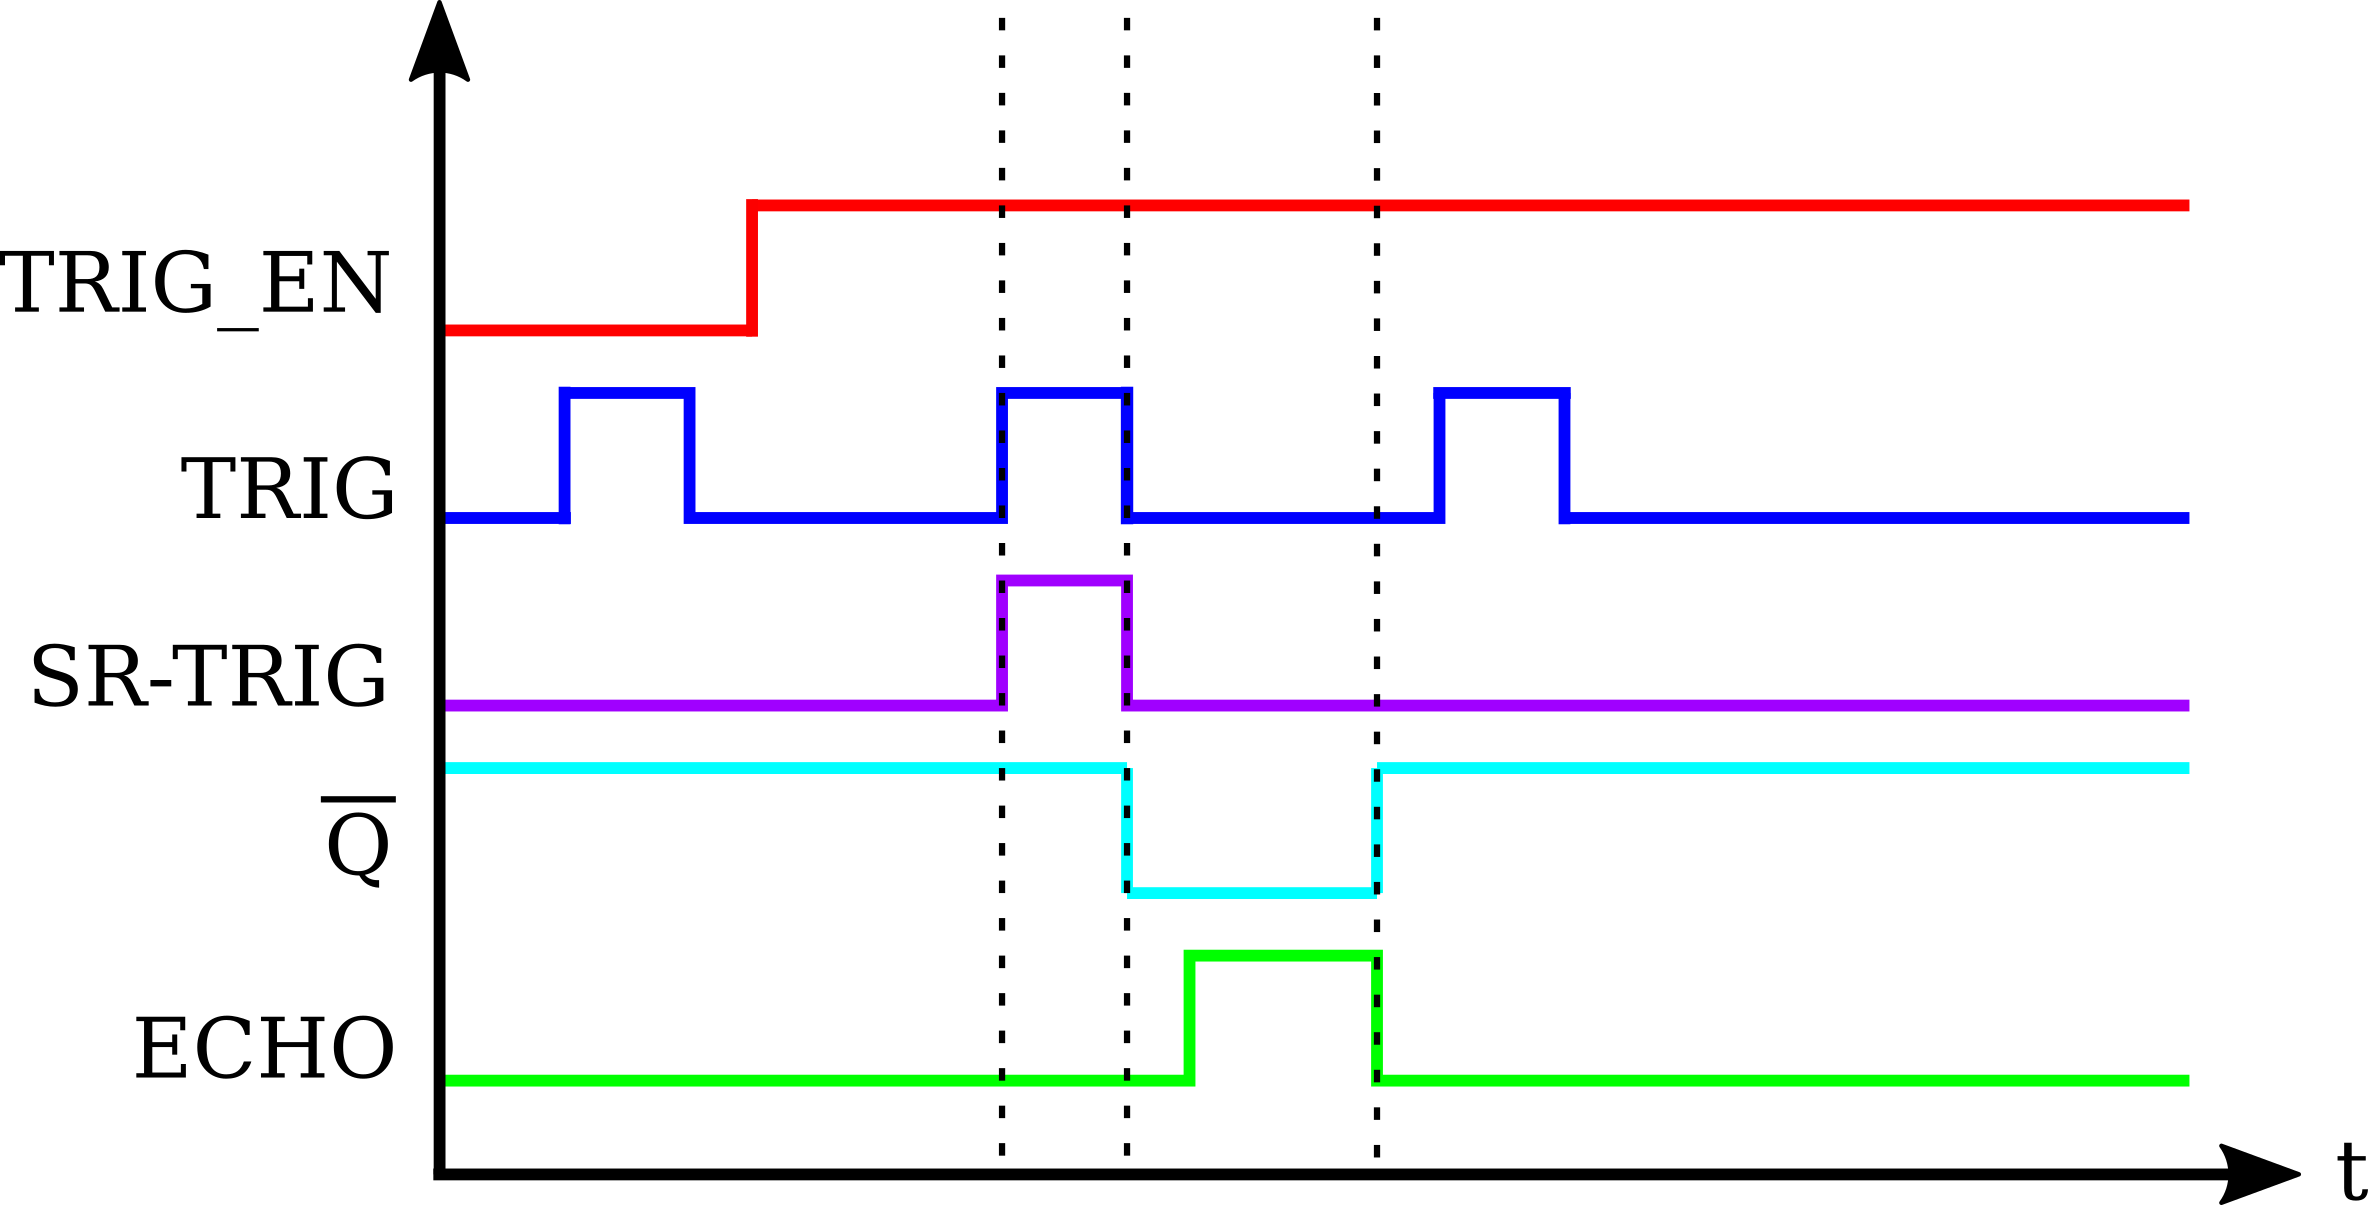
\includegraphics[width=0.7\textwidth]{data/trigerEnable_Time}
    \par\end{centering}
    \caption{Trigger Enable Logic - Time diagram}
\end{figure}
\newpage
The ultrasonic sensor needs a pulse of a period T > 10$\mu$Seg, 
so the edge of TRIGGER input is sended to a monostable circuit
(implemented with a LM555 timer) to ensure that the condition is met.
The final schematic of this section is shown below.

\begin{figure}[H]
    \begin{centering}
        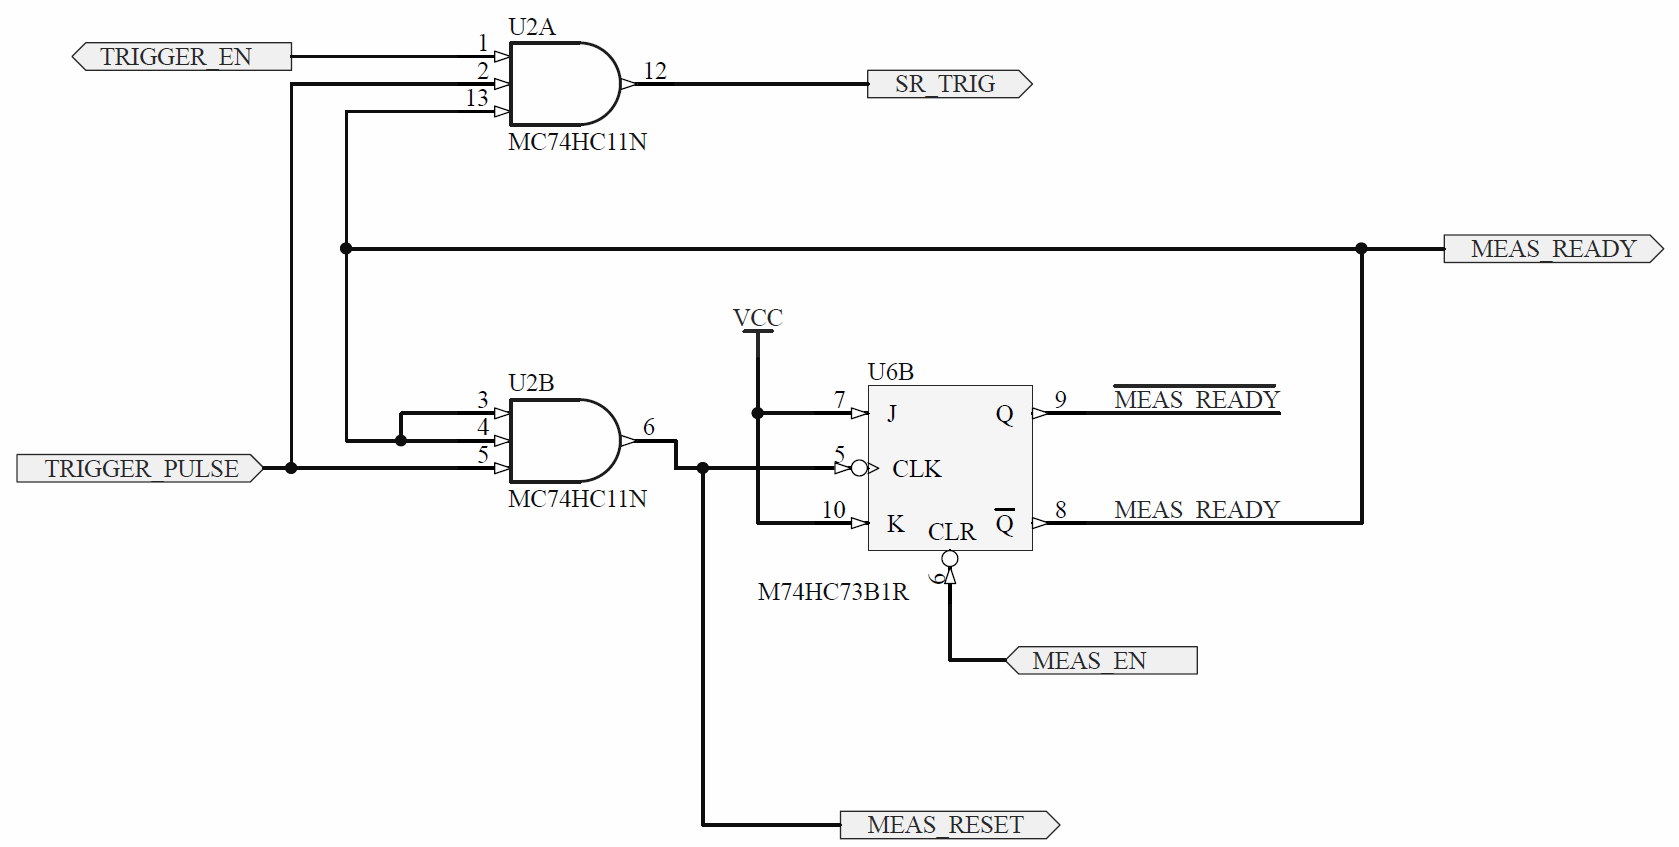
\includegraphics[width=1\textwidth]{data/trig_enable}
    \par\end{centering}
    \caption{Trigger Enable Logic - Schematic circuit made in Altium 15}
\end{figure}

\subsection*{HC - SR04 Sensor}
To make the measures in the mentioned interval, the HC - SR04 
after receiving the TRIG input pulse, it answers at the ECHO out 
with a pulse of a period T > 100$\mu$Seg (1.7cm), up to 25000$\mu$Seg (4.25m).
It will be fractioned in units of 100$\mu$Seg (to be counted).
\par
To know the measure value, the obtained number $N$ is processed in the
following calculation:
\[
    Distance[m] = 170 \cdot 100 \cdot 10^{-6} \cdot N  
\]
By fractioning the ECHO pulse in discrete units, the resulting resolution is
equivalent to 1.7cm, which is the smallest unit that can be counted (100$\mu$Seg).

\subsection*{Measure units detector}

For fractioning the ECHO response into units of 100$\mu$Seg, it is 
connected to an AND gate with a clock source (CLK) whose period is 100$\mu$Seg.\\
In this way, while the ECHO out stays at HIGH level, the signal at the AND gate output 
is equal to the clock source. While not measuring, the output stays at LOW level.
The previous performance is shown in the time diagram below.

\begin{figure}[H]
    \begin{centering}
    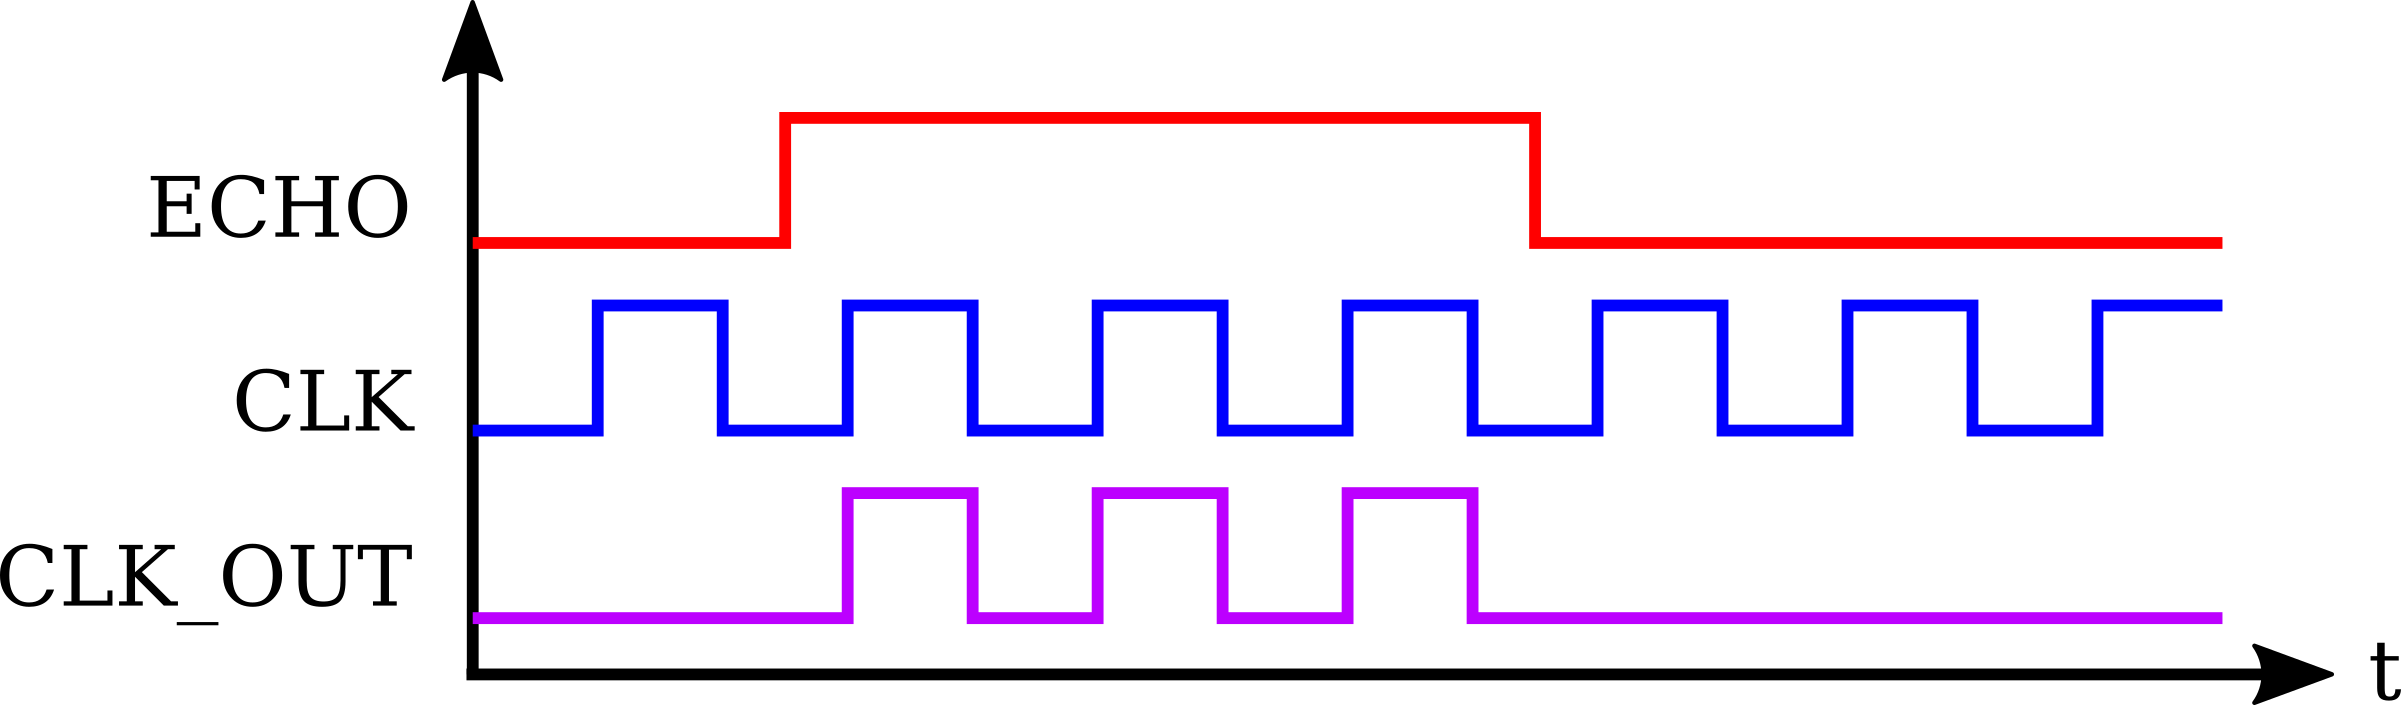
\includegraphics[width=0.65\textwidth]{data/CLK_time}
    \par\end{centering}
    \caption{Measure units detector - Time diagram}
\end{figure}

The CLK signal was implemented with a LM555 timer in astable configuration.
The schematic for this section is shown below.

\begin{figure}[H]
    \begin{centering}
    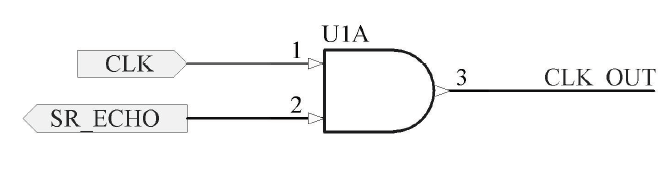
\includegraphics[width=0.6\textwidth]{data/Unit_Detector}
    \par\end{centering}
    \caption{Measure units detector - Schematic circuit made in Altium 15}
\end{figure}

\subsection*{Synchronous counter}

For counting the time units, an integrated synchronous counter is implemented (CD4040), 
whose CLK input is conected to the out signal of the measure units detector. It detects the 
positive edges of the CLK signal, in this case having one per 100$\mu$Seg. From the 12-bit 
output, only 8-bit are used, because for measuring the maximum distance, only 250 untis are 
needed (25000$\mu$Seg over 100$\mu$Seg results in 250 units), and if the binary out is converted 
to decimal, the maximun number is $2^8 = 256$ (which covers the 250 maximum).\\
The integrated circuit implementation is shown below.

\begin{figure}[H]
    \begin{centering}
    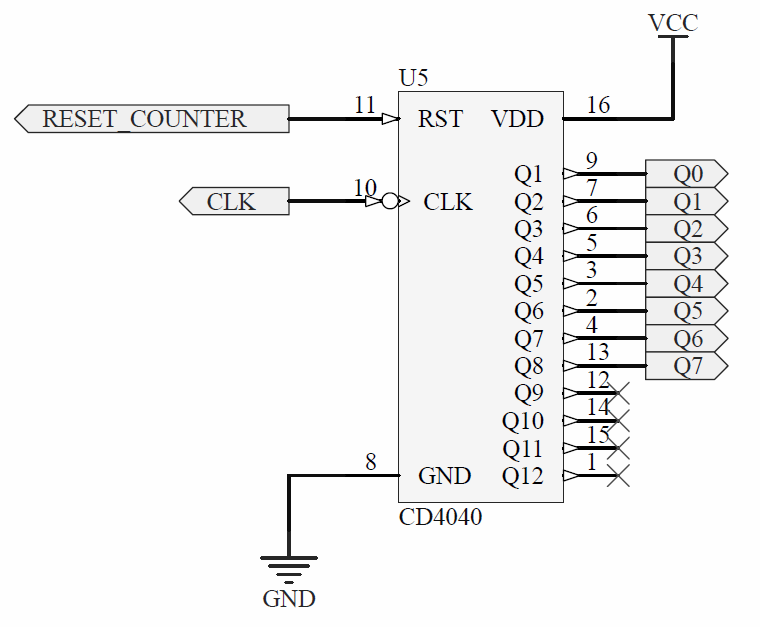
\includegraphics[width=0.5\textwidth]{data/Unit_Counter}
    \par\end{centering}
    \caption{Synchronous counter - Schematic circuit made in Altium 15}
\end{figure}

\subsection*{End of measure detector}

When the measure ends, the negative edge produced by the ECHO is used in a discrete edge detector 
to reset the flip-flop in the trigger enable logic, so a new measure can be started at any time.
The circuit diagram of the implementation is shown below.

\begin{figure}[H]
    \begin{centering}
    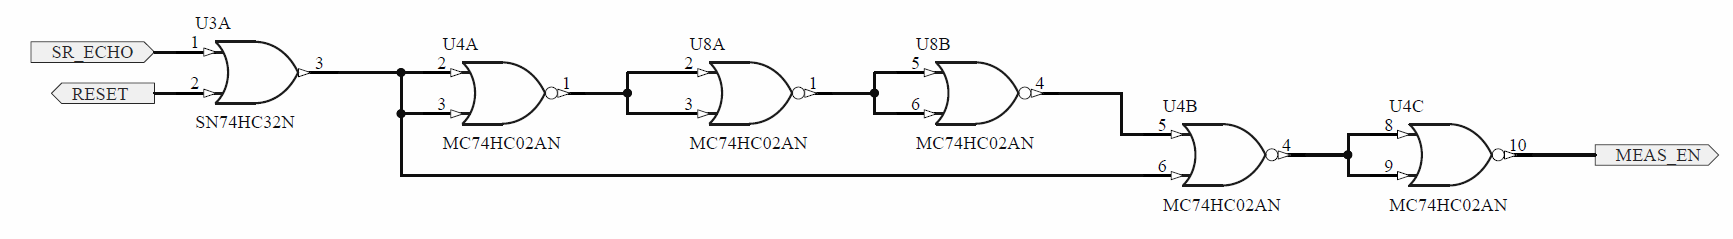
\includegraphics[width=1\textwidth]{data/Meas_End}
    \par\end{centering}
    \caption{End of measure detector - Schematic circuit made in Altium 15}
\end{figure}

The binary output resulting from the measure stays on until a new positive edge from the trigger is 
received. Then, the pulse used to change the flip-flop state in a new measure is also used to reset
the previous binary output from the synchronous counter.

\subsection*{Manual reset}

If when connecting the power supply to the circuit, the counter is not in cero, or the flip-flop starts 
switched into the state $(2)$, a manual switch for reset is added with a pull-down resistor, as shown below.

\begin{figure}[H]
    \begin{centering}
    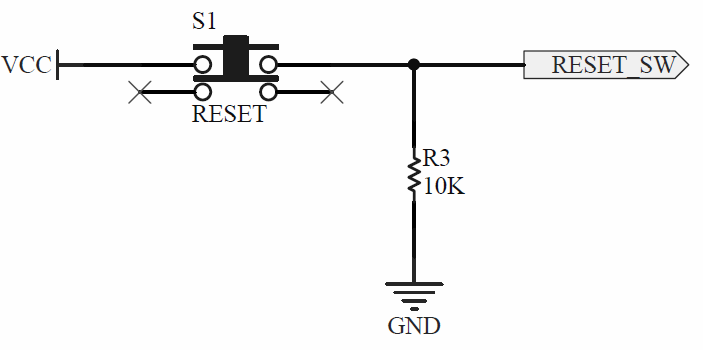
\includegraphics[width=0.5\textwidth]{data/pullDown_Switch}
    \par\end{centering}
    \caption{Manual reset with pull-down resistor - Made in Altium 15}
\end{figure}

\subsection*{Aditional settings}
\subsubsection*{MEASURE\_READY indicator}

To know if the flip-flop starts in the correct state when connecting the power supply or 
if the last measure has finished, 
a bicolor LED was used through two transistors, using the $Q$ and $\overline{Q}$ outputs 
of the flip-flop. When a measure ends (or when at the power supply connection the flip-flop starts
at the correct state), the LED turns green as an OK indication. When measuring, the LED turns red until
it ends. If when connecting the power supply (or in any moment) the flip-flop starts in the 
wrong state, the LED will remain in red. This can be fixed by pressing the reset switch.\\
The schematic circuit is shown below.

\begin{figure}[H]
    \begin{centering}
    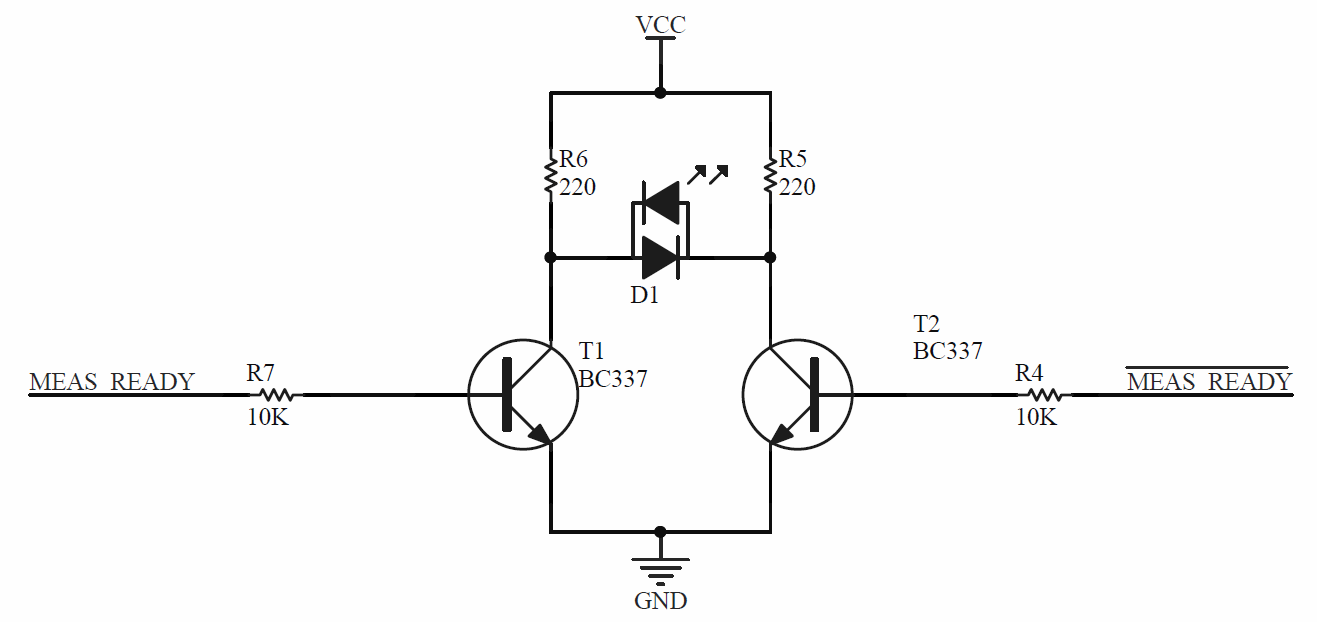
\includegraphics[width=0.9\textwidth]{data/Transistor_LogicLED}
    \par\end{centering}
    \caption{MEASURE\_END indicator - Transistor logic made in Altium 15}
\end{figure}
The calculation of the resistors can be read from the Annex.

\subsubsection*{Measure counted units indicator}

To obtain the amount of time units measured more easily, the CLK out of the
measure units detector is used in decade counters implemented with CD4033, because 
their out pins are decoded for use in 7-segment displays. Since the maximum measure 
has 3 digits, there are 3 counters and displays implemented (their reset pin is 
connected to the reset signal of the end of measure detector, and to the reset switch 
through an OR gate). The implemented circuit schematic is shown below. It has been done in 
a separete PCB.

\begin{figure}[H]
    \begin{centering}
    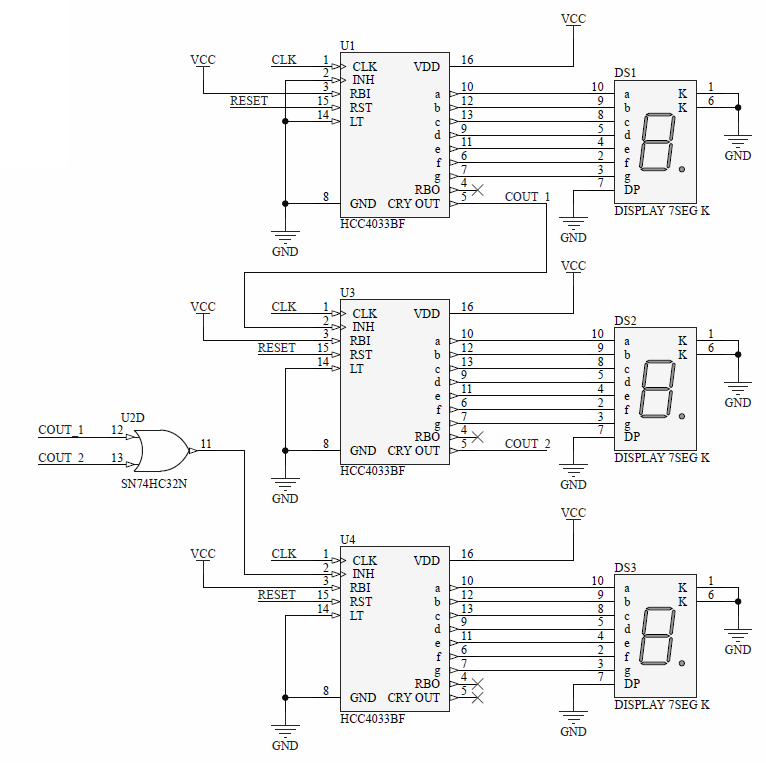
\includegraphics[width=1\textwidth]{data/Display}
    \par\end{centering}
    \caption{Measure display - Schematic circuit made in Altium 15}
\end{figure}

\newpage 
\section*{Appendix}
\subsection*{MEASURE\_READY indicator - Resistors calculation}

For the circuit design, the transistors are used in saturation-cutt off mode. 
Considering a $15mA$ current for the LED, it will be the $IC_{SAT}$. Going through 
the out loop we have:
\[
    V_{CC} - IC_{SAT}R_C - V_{LED} - VCE_{SAT} = 0    
\]
Considering as $VCE_{SAT} = 0.2V$ and a $V_{LED} = 1.8V$, the value of $R_C$ (collector resistor) can be obtained as follows:
\[
    \frac{V_{CC} - V_{LED} - VCE_{SAT}}{IC_{SAT}} = RC = 200 \Omega    
\]
Normalizing the value, it remains as $R_C = 220\Omega $. Recalculating the new $IC_{SAT}$:
\[
    \frac{V_{CC} - V_{LED} - VCE_{SAT}}{R_C} = IC_{SAT} = 13.6mA   
\]
Using the BC337 transistors, according to ON Semiconductor datasheet, the minimum HFE is 100, which will 
be used to calculate the minimum $IB_{SAT}$ (because its the worst case, to guarantee the saturation):
\[
    \frac{IC_{SAT}}{HFE_{MIN}} = IB_{SAT-MIN} = 136\mu A    
\]
With that value, the base resistors can be calculated, and then normalized down to get an $IB_{SAT}$ over 
the previous limit. Going through the entry loop:
\[
    V_{Q-OUT} - VBE_{ON} - IB_{SAT}R_B = 0
\]
Considerating that $VBE_{ON} = 0.7V$ and the output voltage of the flip-flop as $5V$ on HIGH level:
\[
    \frac{V_{Q-OUT} - VBE_{ON}}{IB_{SAT}} = RB_{MAX} = 31.6K\Omega    
\]
Normalizing the value, it results in $R_B = 10 K \Omega$. Checking the resulting $IB_{SAT}$:
\[
    \frac{V_{Q-OUT} - VBE_{ON}}{R_B} = IB_{SAT} = 436\mu A   
\]
According to maximun ratings of Texas Instruments datasheet, the $Q$ and $\overline{Q}$ outs can manage a current
up to $25mA$, so the resulting $IB_{SAT}$ is in range.



